

\subsection{Wave parameters}

\begin{figure}[t]
    \centering
    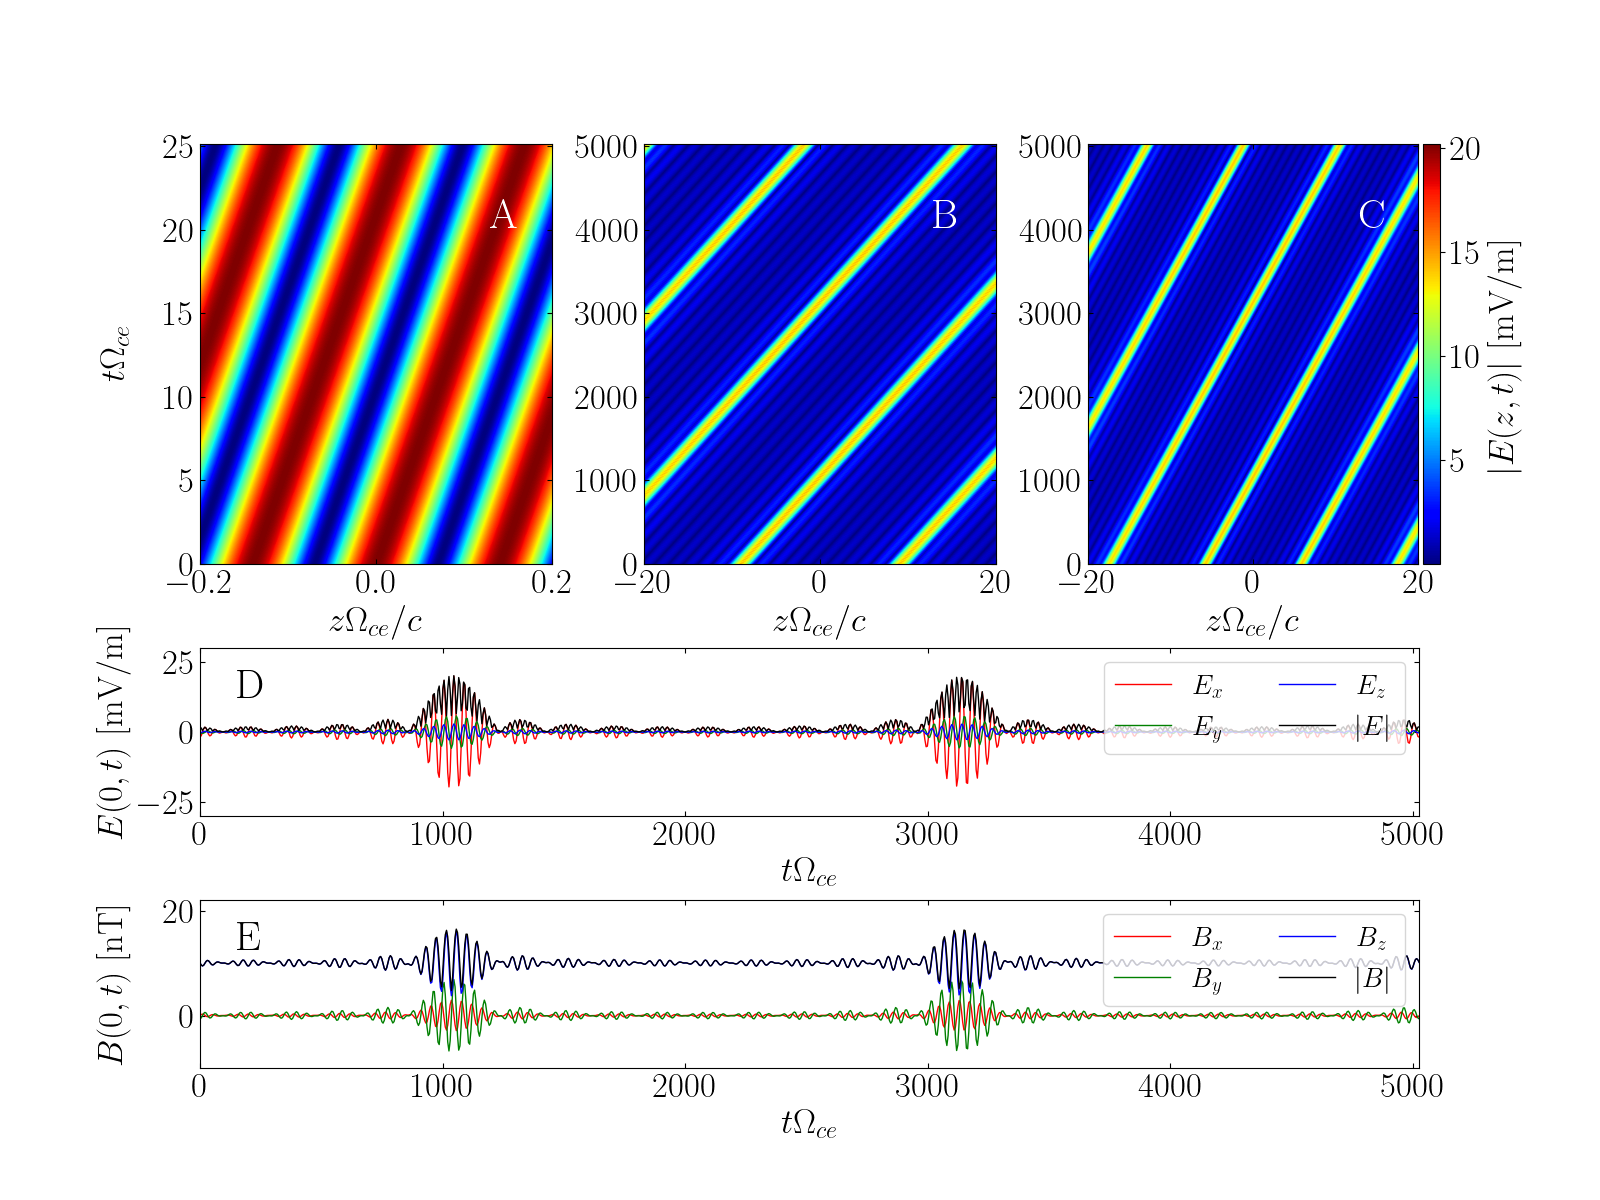
\includegraphics[width=\textwidth]{combo.png}
    \caption{The spatiotemporal evolution at $x=y=0$ of the electric field of an
        oblique ($\theta=65^\circ$) single whistler (A) and oblique whistler
    packets (B \& C). Panels A and B have background parameters for 1 AU and
panel C is for 0.3 AU. Panels D and E show the electric and magnetic field
components at $z=0$ of the packet in panel B.}
    \label{fig:wavefronts}
\end{figure}

In subsequent sections, the interactions of whistlers with electrons in two sets
of background parameters will be studied. The first one is typical of 1 AU with a background field strength $B_0=10$\,\si{nT}. The plasma is quasineutral with $n=n_i=n_e=5$\,\si{cm\tothe{-3}}. The second is consistent with the simulation at 0.3 AU in \cite{Micera2020} with $B_0=50$\,\si{nT} and
$n=n_i=n_e=300$\,\si{cm\tothe{-3}}. The whistler parameters are based on those of \cite{Cattell2020}. For both sets
of background parameters, the single waves have an amplitude
$E_w^0=20$\,\si{mV/m}, frequency $\omega/\Omega_{ce}=0.15$, and propagation
angles $\theta=$ 5, 65$^\circ$, and 175$^\circ$. Whistler packets will contain a
set of eleven $20$\,\si{mV/m} single whistlers with frequency from 0.135 to
0.165 $\Omega_{ce}$ and propagation angles $\theta=0$, $65^\circ$, and
$180^\circ$.

A few examples showing the oblique wavefronts are shown in panels
A, B, and C of \cref{fig:wavefronts}. The phase velocities are different between 0.3 and 1 AU because the background parameters are different. Panels D and E show in more detail the oblique packet in panel B as observed at the origin in time. In \cite{Cattell2020}, the mean observed amplitude was $\si10$\,\si{mV/m}, while those as high as 40\,\si{mV/m} were also observed. Thus, in this study, we use $20$\,\si{mV/m} which has $\delta B_w/B_0\sim0.6$ to clearly see the possible role of the waves. These large amplitude oscillations can result in highly chaotic behavior in the particle motion. Also, note that we are greatly overestimating the parallel wave amplitudes at 1 AU for the sake of comparison. In reality, parallel whistlers at 1 AU are only observed with $\delta B_w/B_0\sim\mathcal{O}(0.01)$.

\begin{figure}
    \centering
    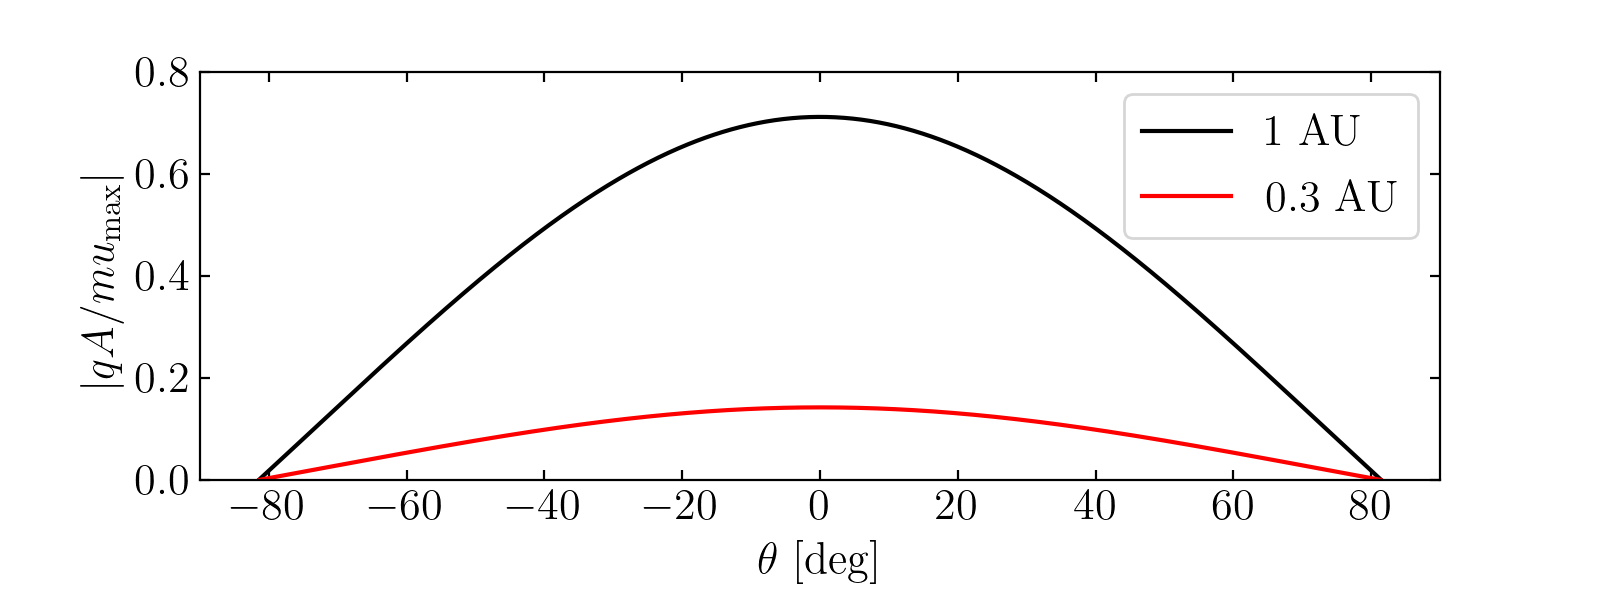
\includegraphics[width=0.95\textwidth]{potential_dominance.png}
    \caption{The ratio between the potential field term $qA$ and the
        particle's relativistic speed term $mu=\gamma mv$ in the canonical
    momentum. $u_{\max}$ corresponds to the maximum kinetic energy of the
simulated electrons. Note that whistlers do not propagate beyond the resonance
cone angle, which is close to 81$^\circ$ but not identical between the black and red
curves \citep{Remya2016}.}
    \label{fig:potential_dominance}
\end{figure}

Since the thermal velocity of electrons in the solar wind is
$\sim2\,000-5\,000$\,\si{km/s}, they are fairly non-relativistic (see
\cref{fig:solar_wind_electrons}). Based on observations of the energy range
for solar wind electrons, particles up to
$\sim$1\,\si{keV} are initiated in the simulations. \cref{fig:potential_dominance} verifies
the small field assumption $\delta_{1,2}<\gamma v/c$ in
\cref{sec:particle_dynamics} for the resonant condition, with $u_{\max}$
corresponding to 1\,\si{keV}. Consequently, $\delta_{1,2}\sim\mathcal{O}(0.01)$
are small compared to unity. So our assumptions regarding the Hamiltonian
derivations are justified, even in the perturbation of these large amplitude
whistlers. For this energy range, the maximum $z$ in our simulations is $\sim30\,000$\,\si{km}, which justifies the assumption of uniform background magnetic field.


\subsection{Particle parameters}

%In a PIC simulation, a weight is attached to each initiated particle, called
%a macroparticle. Each of them resembles a small distribution of electrons and
%together, their motion simulates the evolution of a system of a very large
%number of particles. These macroparticles also have alternated charge, which
%affects the calculation of the charge distribution and consequently the
%electromagnetic field at each time step. However, since we deliberately
%disregard the particles' interaction with the wave and focus on the effect of
%the latter onto the particles instead, we can set their charge to that of an
%electron as is usually done in a test particle simulation. But we will assign a
%weighting function to an adequately large macroparticle distribution to study
%the evolution of electron populations in the solar wind.


As mentioned in \cref{sec:intro}, the two standard velocity distribution
functions (VDF) used to model solar wind electrons are the bi-Maxwellian and the bi-Kappa. The former is
\begin{equation}\label{eq:maxwellian}
    f_M(v_\perp,v_\|)=\frac{n_0}{\pi^{3/2}v_{th,\perp}^2v_{th,\|}}\exp\qty{\qty[\qty(\frac{v_\|-v_{o,\|}}{v_{th,\|}})^2+\qty(\frac{v_\perp-v_{o,\perp}}{v_{th,\perp}})^2]}
\end{equation}
where $v_\|=v_z,v_\perp=\sqrt{v_x^2+v_y^2}$, $v_{th,j}$ is the thermal speed, $v_{o,j}$ is the drift speed in each direction, and $n_0$ is the population density. The bi-Kappa VDF is given by
\begin{equation}\label{eq:kappa}
    f_K(v_\perp,v_\|)=A_\kappa\qty{1+\qty(\kappa-\frac32)^{-1}\qty[\qty(\frac{v_\|-v_{o,\|}}{v_{th,\|}})^2+\qty(\frac{v_\perp-v_{o,\perp}}{v_{th,\perp}})^2]}^{-\qty(\kappa+1)}
\end{equation}
where
$A_\kappa=n_0\pi^{-3/2}\qty(\kappa-3/2)^{-3/2}v_{th,\perp}^2v_{th,\|}\Gamma(\kappa+1)\qty[\Gamma(\kappa-1/2)]^{-1}$. For 1 AU parameters, the core is best modelled by a bi-Maxwellian, while the halo and strahl are best modelled by a bi-Kappa as shown in \cref{fig:solar_wind_electrons} where the maximum kinetic energy is 1\,\si{keV}. The following values are from the mean observations in \cite{Wilson2019}. The initial isotropic core has density
$n_c=13.7$\,\si{cm\tothe{-3}}, zero drift, and
$v_{th}=v_{th,\|}=v_{th,\perp}=1\,800$\,\si{km/s}. The halo is also isotropic
with $n_h=0.52$\,\si{cm\tothe{-3}} and $v_{th}=3\,900$\,\si{km/s}. The strahl
has $n_s=0.21$\,\si{cm\tothe{-3}}, $v_{o,\|}=2\,000$\,\si{km/s}, and
$v_{th,\|}=3v_{th,\perp}=3\,600$\,\si{km/s} (note that it is anisotropic with
$v_{th,\|}\neq v_{th,\perp}$). These VDFs are sampled with
$\sim400\,000$ electrons initiated uniformly in speed with pitch angles (the
polar angle) from 0 to 180$^\circ$ in increments of 1$^\circ$ and gyrophases
(the azimuthal angle) from 0 to 360$^\circ$ in increments of 30$^\circ$. For 0.3
AU, the core and strahl are modelled with the bi-Maxwellian
in parameters similar to \cite{Micera2020}, based on observations by
\cite{Halekas2020} (see \cref{fig:03_AU_particles}). The core has $n_c=332.5$\,\si{cm\tothe{-3}} and $v_{th}=3\,900$\,\si{km/s} with a drift $v_{o,\|}=-480$\,\si{km/s}, while the strahl has $n_s=17.5$\,\si{cm\tothe{-3}}, $v_{th,\|}=7\,900$\,\si{km/s},
$v_{th,\perp}=5\,600$\,\si{km/s}, and $v_{o,\|}=9\,300$\,\si{km/s}.
Approximately a million particles up to 2\,\si{keV} are initiated with the same 
spacing in the solid angle.


